\chapter{Introduction}
\label{ch:Introduction}

\begin{comment}
\setlength{\epigraphwidth}{0.6\textwidth}
%\setlength{\epigraphrule}{0.1pt}
\epigraphhead[70]{%
    \epigraph{It would probably be oversimplifying the
    matter,\\but I am strongly tempted to say,\\ \textquote{All life is nucleic acid; the rest is
    commentary}.}{\cite{asimov:WrongRel}}%
}
\end{comment}

\begin{comment}
When Asimov concluded with these words his chapter \textquote{Beginning with bone},
scientists had already started unfolding one of the most mesmerising biological
mystery: how does the Nature manage and organise the production of specific
effectors in specific locations. In other words how from one cell
\TK{revoir cette phrase: idea initiale pourquoi
organisme A different
de B, ou un foie et un foie et pas un coeur + comment d'une cellule-oeuf on a un
organisme complet qui se creée\ldots ne pas s'étendre dessus par contre}.\
Watson and Crick by publishing the double-helix structure of \DNA\
\mycite{DNA1953} unlocked our path to understand the natural ways of storing and
manipulating the information. As the whole past six decades were packed with major
discoveries and technological achievements, there are many, fascinating,
milestones that could be discussed.
The following pages present a summary of the facts and techniques
that form the biological and technical context of the work backing this thesis.

--- ici intro par rapport à Asimov et le fait que l'ADN est un \enquote{blueprint}
    et qu'en fonction du l'organe ou du develepment stage l'expression est régulé.
    On sait maitenant que la régulation se passe à différent niveau\ldots Finir
    peut être la section sur Harvey qui a élucider la circulation sanguine car
    il a utilisé l'observation et quantification du sang ---


As where the situation stands for now, we know that between the unique common
bluprint, which is the \DNA\ and the different phenotypes displayed by the tissues
comprising our bodies, they are many regulatory processes occurring at different
layers (transcription, and translation).


\Rough{%
Gene expression, transcription, translation, regulation at each stage,
expected and reported correlation between transcripts and proteins
Measuring transcript expression by RNAseq, wet-lab part, analysis methods,
available large scale datasets on human tissues
Measuring protein expression by MS, data analysis – spectral counts, top 3, etc,
available large scale datasets on human tissues
The problem of comparing and integrating independent datasets, EBI’s GXA \\ \\
key concepts: DNA storage, RNA transfert of information and regulation,
protein effectors ==\textgreater phenotype.\\ \\
%
Do not forget the (tissues) specifications and the structural functions. =\textgreater Embryology.\\ \\
%
introduction real possible start: la soupe primaire -\textgreater creation de RNA, aa,
oeuf/poule
premiere cellule, \ldots (lire Darwin, il y a ptet moyen d ajouter une citation ou
    quelque chose).%
}

\begin{itemize}
    \item Proteomics messy and noisy, challenging \ldots
    \item Transcriptomics seem a good proxy to study the phenotype => one kind of molecule made of the same pieces.
    \item Technology improved a lot from the microarrays to sequencing.
\end{itemize}

\end{comment}


\section{Diversity and universality of Life}

\Rough{\begin{itemize}
    \item What we speak about (\gls{DNA},\gls{RNA}, protein)
    \item Why we speak about/study it. Speak of identification of unique features,
        differential expression analysis.
\end{itemize}}

\TK{The central dogma of Molecular biology => Crick describes the cycle}
\TK{add reference on replication? (a priori no review of that part)}

\TK{proteins: polar molecules}


\subsection{Transcription: From \gls{DNA} to \gls{RNA}}
\begin{comment}
Transcriptome is the complete population of \gls{RNA} in a cell or a group of
cells. There are many kinds of them:
\begin{itemize}
    \item \gls{ncRNA}
    \item \gls{tRNA}
    \item \gls{miRNA}
    \item \gls{snRNA}
    \item \gls{scaRNA}
    \item \gls{snoRNA}
    \item \gls{scRNA}
\end{itemize}
\end{comment}

The transcriptome is the total repertoire of transcripts (\ie\ \glspl{RNA}
molecules) expressed in a cell or tissue at a given time and condition. Unlike
the genome which is roughly identical regardless which cell of a particular
individual is considered, the transcriptome varies\ldots

\subsection{Translation: From \gls{RNA} to protein}

\TK{Small conclusion: Assumption mRNA and proteins: highly correlated
[add references]}

\section{Transcriptome exploration with RNA sequencing}

\TK{Two lines about microarrays}

\begin{comment}
Biological research uses mainly two approaches to
study the cell life intricacy and its underlying mechanisms.\\
The oldest approach is descriptive:


Small bits: corrections for Rnaseq are already part of the analysis and
requires often as much flair than skills.
Contrarily to \Dnaseq\ where corrections can be applied \TK{add reference} and
then the analysis be done, in Rnaseq each analysis requires a set of conform
quantification and normalisation methods.
While, there are quite established protocols for differential expression analysis,
there are presently many other downstream analyses that are cumbersome
and/or not settled yet. This is the case for this study.
\end{comment}

With the recent era of short-sequencing technology and the completion of the
Human genome, understanding the genome expression is increasingly a more
reachable aim.
\TK{extend a little}

\begin{comment}
While microarrays are measuring many \mRNAs\ at once, their number is limited,

\TK{history of \Rnaseq.}
In the past decade, \gls{RNA-Seq} technology has risen as the method of choice
for  transcriptome.

Many methods and technologies through the years but more recently, boom of study:
next generation sequencing (1st generation, 2nd generation and 3rd)\ldots So
much that now the expression doesn't mean anything.

Completion of the Human genome project : key changer: probes with microarrays
possible (as there were then template). Next key changer: shotgun sequencing
instead of Sanger sequencing (slow). + advance in computer science: needs of
parallelisation and storage.

So, In 2008, shift from microarrays to \Rnaseq.

\clearpage

\end{comment}

In the following section, I introduce the typical steps of the required workflow
to study the transcriptome through sequencing on an Illumina platform. In fact,
while not by conscious design, all the transcriptomes analysed in this thesis are
the product of Illumina sequencing (see
\crefrange{subsec:castlepresentation}{subsec:gtexPresentation}).
It is not surprising as Illumina was by far
the most popular platform for the last decade \mycite{popularIllumina}.
Indeed, Illumina proposes a very
good ratio between the accuracy and the fact that it achieves the highest
throughput and the lowest per-base cost \mycite{IlluminaCheap}.

Experimental protocols for other platforms will need various and specific
modifications that are outside of the realm of this thesis and thus will not be
cover here\footnote{More details on the other main sequencing platforms and their
relevant protocols may be found in~\cite{rnaseqProtocols} review paper or at the
online resource \enquote{\href{http://rnaseq.uoregon.edu/}{RNA-seqlopedia}}
(\href{http://rnaseq.uoregon.edu/}{http://rnaseq.uoregon.edu/})
\mycite{rnaseqlopedia}.}.

As I discuss the concepts behind the Illumina sequencing technology and the
most common related methods to process it, I will emphasise the approaches and
the tools I used to estimate the gene expression levels from raw nucleotide
sequences.

\Cref{fig:OverviewRnaseqPrepSeq} presents an overview of the typical steps of a
\Rnaseq\ workflow from the libraries preparation to the sequencing.

\begin{figure}
    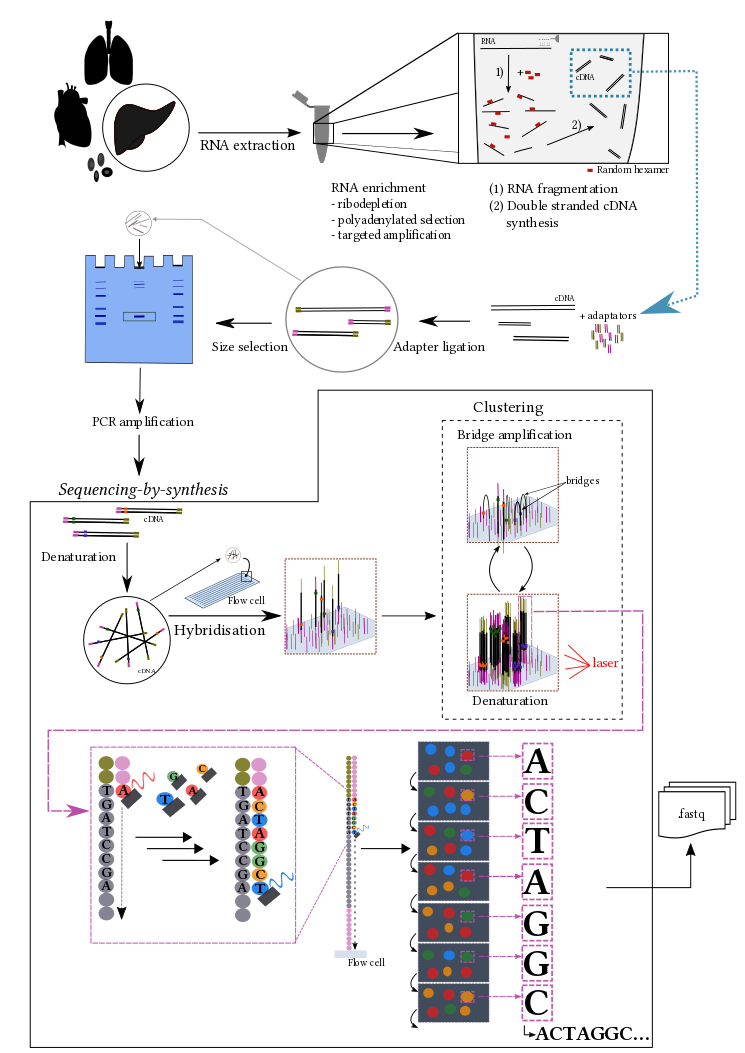
\includegraphics[scale=0.60]{introduction/IntroWorkflow.png}\centering
    \caption[Overview of a \Rnaseq\ workflow: library preparation
    and sequencing]{\label{fig:OverviewRnaseqPrepSeq}\textbf{Overview of
    a typical \Rnaseq\ workflow:
    library preparation and sequencing}}
\end{figure}

\NB\ Albeit the collection and the conservation\footnote{E.g.\ between fresh-frozen
samples and \gls{FFPE} samples see~\cite{sampleConservationMatters}.}
of the samples prior to the
\gls{RNA} extraction most definitely affects the final estimations,
I will let aside these steps from my review.

\subsection{Library preparation}

While there are sequencing technologies that can directly sequence \glspl{RNA}
(see \mycite{rnaDirectSeq}), most of the technologies handle only \gls{DNA}.
Hence, the first step of a typical \Rnaseq\ workflow is the preparation of
\gls{cDNA} libraries from the starting material. This step and the sequencing
itself are the most platform dependent parts of the overall protocol.
Indeed, contingently on to the sequencing principle they rely,
the sequencers need the libraries to be fixed and loaded differently.

\subsubsection{\gls{RNA} extraction}

There are many methods to extract \glspl{RNA} from the primary samples and they
are commonly standardised. Indeed, regarding the type of biological samples,
the \glspl{RNA} of interest, the aim of the  study and the sequencing platform
used, there is one (or more) available commercial kit. These are designed in
a way to not interfere
with any of the later steps of the library preparation or with the sequencing
itself.

Without surprise, the choice of one kit (and hereby method of extraction)
over another can impact the final \Rnaseq\ data. The main difference between
the most widespread methods being the quantity of non-mature \glspl{RNA}
(\ie\ with longer intronic regions) detected whereby kit has been used.
However, the relative gene expression levels are similar from one extraction
protocol to the other. \mycite{RNAextraction}


\subsubsection{\gls{RNA} enrichment}

After extracting the \gls{RNA} from the cells or tissues,
the next step is to enrich the content of the samples with the \glspl{RNA}
of interest (\ie\ the concentration of the \glspl{RNA} of interest is increased
either by specifically selecting it or by removing other \glspl{RNA}). Indeed,
the \glspl{rRNA} are the most abundant type of \gls{RNA} in any cell. Even
though they amount for a very small part of the genome\footnote{For example,
\species{Homo sapiens}, there are 568 genes (<1\%) that are described as
\gls{rRNA} out of the 63,898 annotated genes of the \gls{Ensembl} database
(\hg{38.p10}, \ens{89}).}, they represent by their number 70\% or more of
the total population of \gls{RNA} \mycite{biochbook}.
Although there are interests to study \glspl{rRNA} (\eg\ \mycite{rrnaStudy}),
\mRNAs\ studies are more
popular and they only constitute about 3 to 5\% of the whole \gls{RNA} population
\mycite{molBiolCell}. Other studies research even scarcer kinds of
\gls{RNA}.\footnote{Out of the 10,081 experiments tagged as \comp{\enquote{rna
assay}} and \comp{\enquote{sequencing assay}} within \gls{ArrayExpress},
7,981 were also tagged as \comp{\enquote{RNA-seq of coding RNA}},
1,829 as \comp{\enquote{RNA-seq of non coding RNA}} and 366 have both tags.
4 of them are only described as \comp{\enquote{microRNA profiling by
high-throughput sequencing}} --- Query date: 22 June 2017.}

There are typically three strategies to achieve \gls{RNA} enrichment:
either by polyA-selection, by ribodepletion or (more complex)
by targeted amplification. While these
approaches are insufficiently specific to select one particular kind of \gls{RNA}
or remove all \glspl{rRNA}, it eases and improves the downstream analyses.

\minisec{PolyA-selection}
This strategy essentially targets the \mRNAs. It exploits the polyadenylated
tail at the 3' end of the \mRNAs\footnote{And a few other kinds of \gls{RNA},
\eg\ \glspl{lncRNA} \mycite{polyAlncRNA}} that is added
post-transcriptionally. In fact, magnetic beads supporting short
strings of thymine (oligo-dT) capture efficiently these \mRNAs\ while the others
are washed away \mycite{Mortazavi2008}.

This protocol is probably the most widespread one as it is the easiest and
cheapest to set up. A dataset produced following this protocol is known as
a \emph{polyA-selected} dataset.

\minisec{Ribodepletion}
This strategy is preferred for the study of any \gls{ncRNA} or when researching
the interaction of \mRNAs\ with other \glspl{RNA} \mycite{ribodepletion}. This
strategy is in a way the reverse of the previous one as its also
uses magnetic beads, but this time to efficiently\footnote{ThermoFisher claims
that its RiboMinus protocol can remove till 99.99\% of the \glspl{rRNA}.}
target the unwanted \glspl{rRNA} as to remove from the sample.

The ribodepletion can also be achieved through ribonucleases. These enzymes
specifically digest \glspl{rRNA} and then \glspl{RNA} of interest can be retrieve
through size selection.

Datasets produced following a ribodepletion protocol are usually called
\emph{whole \gls{RNA}} or \emph{total \gls{RNA}} as a contrast to the
\emph{polyA-selected} ones.

\cite{castleData} created a total \gls{RNA} dataset but they use another
approach where they amplify \emph{every} other \gls{RNA} with the help of
specifically designed probes (see \cref{subsec:castlepresentation}). Hence,
the protocol they have used is closer to the following one.

\minisec{Targeted amplification}
Targeted amplifications rely on primers that would be designed to target (or
avoid as for~\cite{castleData}) specific sequence motifs of the genome. Most
studies based on this kind of approach are not referred as \Rnaseq\ studies, but
a name that is based on the studied \gls{RNA} type (\eg\ \gls{miRNA-Seq}) or
that emphasises the variation of the method (\eg\ Capture-Seq
\mycite{captureSeq}). Often, in comparison with a polyA-selected or ribodepleted
dataset, additional steps are required to prepare the libraries.


\subsubsection{RNA fragmentation}

Most of the sequencing platforms\footnote{As for the Illumina platforms that have
produced the transcriptomic datasets studied in this thesis.} require relatively
short (\ie\ 200 to 500\ nt) length to sequence. Concomitantly, it also ensures
that the sampling along the \gls{RNA} is more uniform.
This fragmentation can be carry out via divalent cations hydrolysis or
nebullisation.

This step is performed on occasions after the \gls{cDNA} synthesis
(see next section). In those case, the \gls{cDNA} are fragmented mostly
by digestion with DNase I or by sonication.

\subsubsection{Double-stranded cDNA synthesis}
The \gls{RNA} molecules are used as a template for a retro-transcription
involving oligo-dTs or \emph{random} hexamer primers, respectively only
for polyA-selected datasets or any dataset (polyA-selected included).
The set of \emph{random} hexamer has been designed to cover the whole
transcriptome. Unfortunately, these \emph{random} hexamer primers have been
proven to actually lack full randomness \mycite{notSoRandom}.

At the end of the most common protocol, the order of synthesis of each \gls{cDNA}
strands is lost, \ie\ it is impossible to distinguish which of the \gls{cDNA}
strands has the same sequence than the original \gls{RNA}. Several techniques,
called \emph{strand-specific}, have been developed to compensate for this
(\mycite{strandSpecific}, \mycite{strandSpe}).

\subsubsection{Adapter ligation, PCR amplification and size selection}
After generating blunt edges by restriction digest of the \glspl{cDNA}, adapters
(small known sequences of oligonucleotides) are ligated to their both ends.
These adapters are constituted from several parts. A subset of them are ensuring
later the hybridisation of the \glspl{cDNA} with the flow
cells\footnote{\Gls{flow}: see \cref{sub:HybridClustAmp}.} (based on sequence
complementary) and another set of them
are sequence binding sites that are used as primers for the following cluster
amplification step occurring \latin{in situ}. These adapters are also used to
introduce additional motifs such as indexes.

The next two steps can be interchanged regarding the amount of starting material
at disposition. All the molecules are amplified by \gls{PCR} before (or after)
a size-selection is performed (per gel electrophoresis) to extract
length-complying fragments (about 200 to 500\ bp) to the sequencer machine
requirements\footnote{Indeed, the previous fragmentation step creates a great
length range of fragments.}.

Unfortunately, the size-selection means that any
transcript with an original length below the threshold used for the
selection will be missed\footnote{There is no problem for the greater length
as statistically they will present fragments that will be in the correct range.}.
For example, \glspl{miRNA} are shorter than the general requirement of Illumina
sequencers. Alternative protocols are addressing this issue
\mycite{smallRNAprotocol}.

\subsubsection{An example of alternative preparation strategy}
Along with the targeted, the strand-specific and small \glspl{RNA} protocols,
there are a few other variations to this typical protocol to handle other concerns.
For example, it is occasionally necessary to sequence simultaneously (in a single
run) multiple samples. This can be motivated by practical reasons
(to lower the experimental costs or hasten the overall processing time)
\mycite{multiplexCheaper} or critical to the experimental design as a way to
experimentally handle the \emph{batch effects}\footnote{Batch effect: see
\cref{sub:BatchEffect}} \mycite{multiplexBatchEffect}. However, it is
crucial to later extricate the several pooled samples from each other as a
requirement to many downstream analyses.

\emph{Multiplexed} protocols easily achieve
the distinction between the multiple samples as they incorporate \emph{barcodes}
before ligating the adapters. These barcodes are also small sequences of
nucleotides and each sample has its own unique associated
barcode. In practice, each sample is prepared separately with the added extra
step (before the adapters ligation) where the barcode is incorporated, then all
the samples are pooled together before the next step that consists to hybridise
the \glspl{cDNA} to the flow cell.

Other extra steps occur just after the sequencing and before any other data
analysis: all the reads\footnote{Reads: see \cref{subsub:sequencing}} are
separated in files based on their barcodes and the barcode, along with the
adapters, is trimmed from all the reads.

The main inconvenient of the multiplexing protocol is that the original sequenced
length of the \glspl{cDNA} are then shorter as the barcodes are also (and have
to) be sequenced as well.

\subsection[Clustering: Hybridisation and Bridge amplification]{Clustering:
Hybridisation and Bridge amplification \mycite{IlluminaYoutube}}
\label{sub:HybridClustAmp}

Once the libraries are ready, they are loaded onto a \emph{flow cell}\footnote{%
\emph{Flow cells} are the support of Illumina sequencing. They enable the
parallelisation of the sequencing of millions of \gls{DNA} fragments together
which are kept spatially separated in clusters. This was allowed with the advent
and optimisation of supported Chemistry. Each flow cell is a glass slide with
lanes. Each lane is coated with two short nucleotide sequences. One of these
oligonucleotides is complementary to a region comprised in the ligated adapters.}.

The clustering step comprises two phases: hybridisation and bridge amplification
of the \gls{cDNA} fragments.

\subsubsection{Hybridisation}

The double-strand \glspl{cDNA} are denatured and then each fragment randomly
hybridises across the flow cell surface with one of its small oligonucleotides.
These are used as primers for polymerases which create a first complementary
strand to the hybridised \gls{DNA} fragments. The new double-strand molecule is
denatured and the original first template is washed away.

\subsubsection{Bridge amplification}
The strands then folds over and their (second) adapter hybridises with a
complementary oligonucleotide sequence of the flow cell and thus creating a
bridge. The flow cell complementary fragment is then used as the primer for a new
strand. The new double-stranded \gls{DNA} is then denatured (which
dismantles the bridge). Each of the two tethered molecules creates a new
bridge by hybridisation which are the templates for a new strand each.
This process happens many times and simultaneously for millions of fragments.
It creates clusters of clonal amplification of the original fragments of
the library. After the bridge amplification, the reverse strands are cleaved
and washed away. The 3' end primers are also blocked to avoid any unwanted
priming.

\subsection{Sequencing-by-synthesis}
\label{subsub:sequencing}

Illumina sequencers propose two sequencing approaches: single-end and paired-end.
The difference is that in \emph{single-end sequencing}\footnote{Chronologically
the oldest method}, the sequencing begins at one (and only one) of the fragment
ends and progresses towards the second. Whereas in \emph{paired-end sequencing},
once the first end has been sequenced (as in the single-end approach), after a
single new bridge replication, the other end of the original fragment is
sequenced as well. Hence, in paired-end, the sequencing occurs at \emph{both}
ends of each original fragment. This has been allowed by a small change in
the original single-end adapters \mycite{pairedEndAdapters}.

Though more expensive and more challenging to programmatically handle,
the paired-end approach produces more information and hence facilitates
the detection of genomic rearrangements (as indels or inversions) and
repetitive sequence elements.
It also allows an easier distinction between isoforms of a same gene and provides
greater support to the novel transcripts (new isoform or new gene) and fusion
genes\footnote{A \gls{fusionG} is a gene that is the product of the fusion of
parts of two different genes.}.

In both cases, the sequencing process is the same. It is an Illumina proprietary
process and it is called \emph{Sequencing-by-Synthesis} \mycite{seqBySynth}.
It uses the \gls{DNA} replication mechanism with modified \dNTPs.
It relies on the step-by-step incorporation of
reversible fluorescent tagged \dNTPs\ who are protected at
their 3'end to block any further elongation.
The product of this synthesis is called a \emph{read} and it supports the base
calling.

The sequencing occurs simultaneously on every identical fragment
of every cluster of the flow cell.
It begins with the hybridisation of a complementary 5' primer onto the 3' biding
site of the tethered \gls{DNA} template. This primer is then extended by
replication to create a new read. Next, the sequencing cycle (described below)
repeats itself several times.

The \emph{sequencing cycle} starts with the addition of one complementary
fluorescent \dNTP\ to the new growing read and, since the \dNTPs\ are blocked at
their 3' end, the replication process stops. Afterwards, all the unlinked
\dNTPs\ are washed away. Then, the clusters are excited by a light source
and as each
\dNTPs\ has a fluorescent tag with its own characteristic wave-length, the
signal that they emit back will allow to \emph{call} (\ie\ identify) what is the
new nucleotide that each cluster has incorporated. The signal intensity, along to
its wave-length are recorded (both of them are needed for the base calling
process for the base call itself and its associated accuracy). Finally,
the fluorescent tags and the 3' caps are cleaved
and washed away so a new cycle can happen.
The number of cycles determines the final length of the reads.

Unfortunately, as the sequencing proceeds, the error rate of the sequencers
increases. This is due to the incomplete removal of the fluorescent signal which
increases the background noise and thus reduces the signal-to-noise ratio.

Once the programmed read length is achieved (typically between 25 to 200 \gls{nt}),
the reads are washed away (after denaturation).

\subsubsection{Sequencing specificities for the \emph{paired-end} protocol}

Then, after introduction of a new primer, the first index is sequenced
following the same sequencing cycle.
Once completed, the index read is washed off and the 3' end primer is deprotected.
Then, the \gls{DNA} fragment bends over and hybridises to a complementary
oligonucleotide at the surface of the flow cell.
Next, the second index is sequenced and its product read washed away,
a single new bridge replication follows.
The new double-stranded \gls{DNA} fragment is denatured and the 3' primers are
protected before the forward strand is cleaved and washed away.
Finally, the reverse strand is sequenced following the previously described
sequencing cycle. Once the same number of sequencing cycles than the forward
strand is reached, the read product of the reverse strand is washed away.

\subsection{From analogous input to digital output}

At the end of the sequencing process, the set of images (one per sequencing cycle)
is produced. While it is possible to work with the images themselves, in most
cases, the sequencing facilities will perform the base calling and provide the
end-user with text files. In single-end sequencing, there is one file per sample.
In paired-end sequencing, the reads are separated based on their associated
indexes into two ordered files: all the reads from the forward strands (one end)
are grouped in one file, and the ones from the reverse strands (other end)
in another.

These files are usually distributed in \fastq\ format
\mycite{fastqFormat} which record for each cluster (read) a unique identifier,
a nucleotide sequence and a \gls{Phred} quality score for each base of the
sequence. A few optional information can also be provided (\eg\
the position of the read on the \gls{flow} (See \cref{sec:fastq_format} for
a random read example).

The \gls{Phred} quality score ($Q$) measures the accuracy of the identification
of the nucleobase to which it refers. These score are set by the base calling
program and are defined as $Q = -10\log_{10}(P)$ with $P$ the probability of
the base being called wrongly. There are several possible encoding formats
(see \cref{sec:PhredScore}).

\subsection{A typical bioinformatic workflow for \Rnaseq\ study}

From the reconstruction of the
transcriptome to the normalisation of expression in each sample, the various
steps may be addressed through a number of different algorithmic approaches.
Often, the choice of a method at one stage implies a more limited number of
alternatives from which to pick at later points in the pipeline. Actually,
the choice is frequently driven by the kind of downstream analyses planned for
the study. More than the practical format of the data for these, it is the
assumptions and the correction methods used upstream that are critical for a
rigorous investigation and, later, for an accurate interpretation of the results.

\Cref{fig:pipelineTrans} present an example of the overall \latin{in silico}
process of raw \Rnaseq\ data. It summarises the steps and highlights the tools
I used to process the data within this thesis.

Before any downstream analysis, for each read, the genomic region (or
\emph{locus}) from which it has been originally expressed need to be identified.
Indeed, \Rnaseq\ main objective is to quantify the expression of genomic
\emph{features}\footnote{These genomic features could be genes, isoforms,
exons, novel genes, \dots\
In short, any genomic region with an annotated function.}. In other words,
the transcriptome needs to be reconstruct from the short reads and annotated
(\ie\ identify which features have been expressed in each library).

Two main different strategies (see further `Reconstruction strategies' segment)
manage to accomplish this identification step. Independently of the
approach, this step is the most challenging and time consuming
of the workflow. Tools, that tackle the reconstruction, usually provide a
number of tunable heuristic parameters (\eg\ maximum number of allowed mismatches
or indels per read before discarding a possible identification\footnote{Indeed,
many reads will have many identifications, these reads are defined as
\emph{ambiguous reads}.})
to speed up the task.
Unfortunately, as on Illumina platforms, the base calling accuracy decreases
along the read length, this may lead to an information loss \mycite{TrimRNAseq}.
To prevent informative reads to be discarded, it is opportune to perform a quality
check of the raw data prior to the identification step. Thus, reads with a drop of
accuracy in their 3'end may be shortened (\ie\ trimmed) and rescued for the next
reconstruction step. Similarly, low quality reads may be discarded hence
lowering the complexity
of the reconstruction task and hasten its accomplishment.

\subsubsection{Quality check, trimming and filtering}\label{subsub:trim}

The quality assessment allows to remove any read (or part of it) that would
increase the complexity of the reconstruction step or skew the downstream analyses.

It is wise to discard uninformative reads, \ie\ reads with a low sequence
complexity (\eg\ poly-T or poly-A tails) or with ambiguous sequences (in other
words with uncalled bases --- reported as \emph{N}).
Indeed, these reads will hamper the processing time as they
usually map to several parts of the genome while also decreasing the accuracy of
the global gene expression estimations.

For similar reasons, it is judicious to remove reads with a low overall quality
score\footnote{It may vary based on the complete set of reads to analyse.}.

It is also prudent to check and remove any read that may map to possible
contamination sources\footnote{For example, for eukaryotes, by aligning (see next
segment) every read to the \species{Escherichia coli} genome}).
Indeed, as these reads are ambiguous, it is safer
to discard them than skew the expression estimations.

Finally, as a number of tools (mappers in particular) only accept reads
with an unique length, the purity-length balance requires optimisation.
Indeed, the trimming has to compromise between
an approach too lenient (where many unfit reads are discarded
by the mappers at a later step) and
a too stringent one (where too little reads are left for a pertinent analyses or
where shorter reads increase the overall complexity and therefore hinder
the mapping both on time and accuracy \mycite{Trimwisely}).

\NB\ Generally, after the sequencer calls the reads, a first trimming removes
all the adaptors and barcodes needed by the sequencing protocols. Thus,
in principle, they are not to be found in the \enquote{raw data}.
However, to avert any latter contingency, a research against
a list of the most common adaptors and an over-representation assessment of small
sequences (\emph{k-mers}\footnote{\emph{k-mer}: In the present context, all
possible subsequences of length
\emph{k} of a \emph{read}.}) at each end of the reads is good practice.


\subsubsection{Reconstruction strategies}

Two main approaches can be used for the very computationally expensive step of
identification. I will present them in a decreasing order of complexity:
the \latin{de novo} assembly of the reads and then the Reads alignment approach
(to a genome reference or a transcriptome one).

Regardless of the approaches, the reconstructed transcriptome is usually reported
as a \emph{\gls{SAM}} file \mycite{SAMformat} (or one of its derivative format
either \emph{\gls{BAM}} or more recently \emph{CRAM}).

\begin{comment}
\begin{figure}
    \includegraphics[scale=0.60]{introduction/MappingStrategies3.pdf}\centering
    \caption[Overview of main reconstruction strategies for
    \Rnaseq\ transcriptome]{\label{fig:OverviewRnaseqMapping}\textbf{Overview of main
    reconstruction strategies for a \Rnaseq\ transcriptome}}
\end{figure}
\end{comment}

\minisec{\latin{de novo} Assembly}
This approach is favoured when the reference genome of the species of interest
is unavailable or of poor quality
(\eg\ many non-model organisms) or inadequate (\eg\ cancer samples)
for the samples of interest. However, if a reference already exists this strategy
is avoided to the utmost.

It allows the unbiased discovery of novel
exon-exon junctions \mycite{deBruijn}. As none of the datasets I use in this
thesis has been reconstructed through this approach, I briefly summarise
the main points below as more in-depth reviews cover this strategy
\mycite{denovoReview}.

In \latin{de novo} assembly, the reconstruction of the transcriptome happens
with the construction of the longest possible \emph{contigs} (\ie\ contiguously
expressed regions) based on sets of overlapping reads (see also
\Cref{fig:denovo}). Short length reads add
to the overall complexity of this approach. While paired-end reads may help to
solve a number of genomic regions, lowly expressed or repetitive regions remain
challenging to determine. There are several algorithmic approaches for \latin{de
novo} transcriptome assembly \mycite{algorithmsDenovo},
though the most prevalent one is the de Bruijn representation \mycite{deBruijn}.

\begin{figure}
    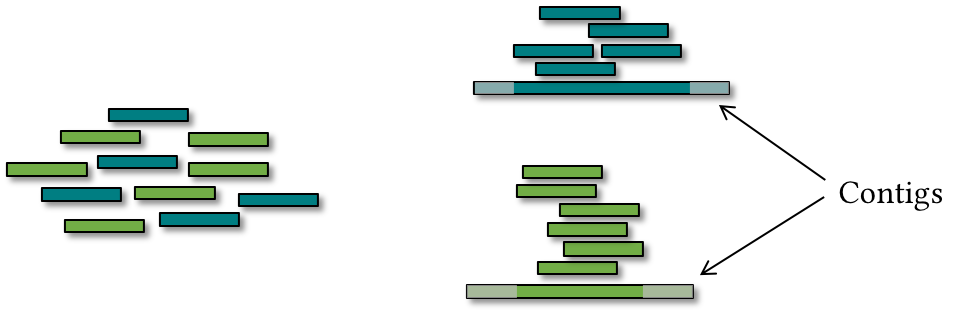
\includegraphics[scale=0.60]{introduction/denovo.png}\centering
    \caption[\textit{de novo} Assembly]{\label{fig:denovo}\textbf{\latin{de novo}
    Assembly.} From overlapping regions of raw reads, \emph{contigs} are
    created by integrating the reads sequences together.}
\end{figure}

\begin{figure}
    \centering
    \begin{subfigure}{1.1\textwidth}\label{fig:genoAlignment}
        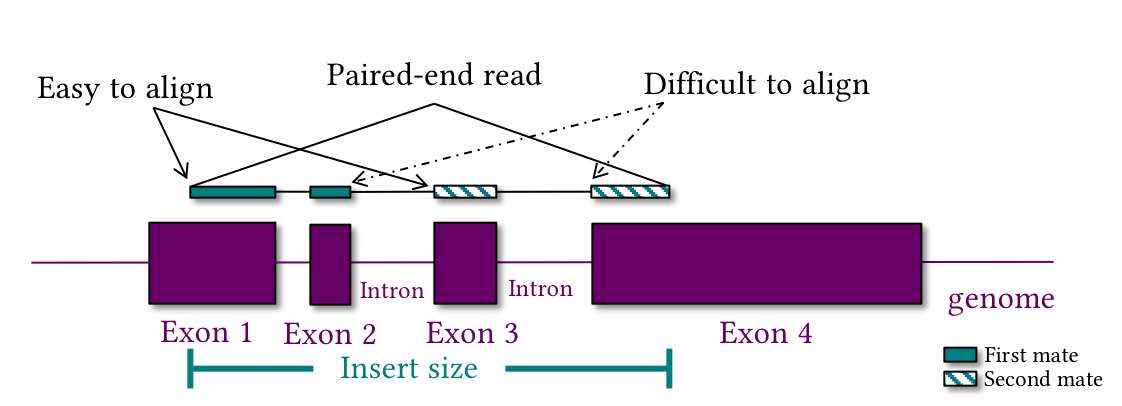
\includegraphics[scale=0.60]{introduction/genomeAlignment.png}\centering
        \caption{Alignment to the genome}
        %\label{fig:genoAlignment}
    \end{subfigure}

    \begin{subfigure}{1.1\textwidth}\label{fig:transAlignment}
        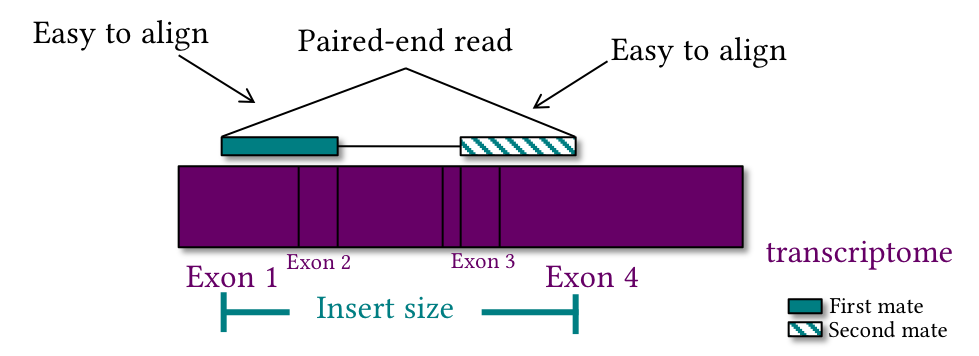
\includegraphics[scale=0.6]{introduction/transcriptomeAlignment.png}\centering
        \caption{Alignment to the transcriptome}
        %\label{fig:transAlignment}
    \end{subfigure}
    \caption[Overview of main alignment strategies for \Rnaseq\
    transcriptome]{\label{fig:OverviewRnaseqMapping}\textbf{Overview of main
    reconstruction strategies for a \Rnaseq\ transcriptome by alignment to a
    reference}}
\end{figure}


\minisec{Read alignment}
This approach exploits prior knowledge. The reads are aligned to a reference to
hasten the reconstruction process. The reference may be a genome or a
transcriptome (provided that a good annotation is available).


\subminisec{Genome reference}
Aligning to the genome allows to discover new genes or isoforms. However, it
requires a splice-aware algorithms, \ie\ they need to align the
reads across the splice-junctions (which is possible but non-trivial).
As illustrated in \Cref{fig:genoAlignment},
the reads might span a number of discontinued regions of the reference.
While on one hand, aligning to the genome avoids \emph{multiple mapping
issues}\footnote{Due to sequence similarity, a same read or subpart of a read
may be attributed to a number of different loci in the genome. As it is
impossible to directly attribute the read to its original locus of expression,
distribution models have to be pondered to avoid unnecessary skewness while
the quantification step.} for a same exon. Indeed, irrespectively of the number
of a gene isoforms including an exon, the sequence of this exon is transcribed
only once in the reference. However, this also implies that, for correct
quantifications of the different isoforms, the genome needs to provide the
coordinates for the isoforms and that an accurate quantification at isoform levels
requires further analysis.

\subminisec{Transcriptome reference}
Using a transcriptome as reference instead of a genome reduces the complexity
of the aligning step due to the lack of intronic sequences. However, it also
limits the potential downstream analyses, \eg\ any new (or unannotated) gene
or isoform will be missed. This approach is the easiest, but a pre-existing
accurate and well-annotated gene models is required.
\Cref{fig:transAlignment} shows in fact that this approach is simpler
to the previous one as a direct alignment of the reads is done against the
transcriptome of reference. This enables to quantify accurately the expression
of gene isoforms, provided that the gene model is correct and the reads may be
attributed unambiguously to a single isoform for each gene.

To mitigate between very computational greedy approaches and more constraining
ones, several tools complementary use the previous strategies.

\minisec{Hybrid approach between \latin{de novo} and alignment}
There are tools like \toph\footnote{\toph\ ---
\href{https://ccb.jhu.edu/software/tophat/index.shtml}
{https://ccb.jhu.edu/software/tophat/index.shtml}} (2.0.12) \mycite{tophat2}
(which has been used to reconstruct all the
transcriptomes involved in this thesis --- see \Cref{ch:datasets}),
that uses an hybrid approach between a reference alignment and a \latin{de novo}
assembly. As a first (but optional) step, \toph\ tries to contiguously
align the reads with \soft{Bowtie}\footnote{\soft{Bowtie} ---
\href{http://bowtie-bio.sourceforge.net/index.shtml}%
{http://bowtie-bio.sourceforge.net/index.shtml}} \mycite{Bowtie}
to the reference transcriptome when this one is provided. Then
(or alternatively as a first step), the unmapped reads are aligned to the
reference genome. The intention in these alignment steps is to identify and
localise the exons, which may eventually span over splicing junctions and be
connected through spliced alignment. Then, \toph\ builds a database of
possible exon-exon splice junctions from the set of mapped reads and then split
the remaining unmapped (or aligned with a low score) reads to smaller segments
in order to find
possible new split events via a seed-and-extend approach. Potential new events
are considered when these smaller segments, first, match exactly the reference
for their regions with good quality score and, secondly, they have overlaps
(for an user defined length) with a splice junction. These segment sections are
called seed. Any read with a seed is then checked for a longer or even complete
alignment to the exons on both side of the junction.

In the case of paired-end data, each read of the pair is first processed
separately. Then, they are a valuable resource as a pair in the final evaluation
phase, where with additional
information sources, they help to determinate among the many possibilities which
are the most credible ones. Both part of a paired-end data once aligned to a
concordant region of the genome is then called a \emph{fragment} instead of a
\emph{read}. Nowadays, there is an assimilation between the \enquote{\emph{read}}
and the \enquote{\emph{fragment}} terms. Even though, the locution \emph{fragment}
is more accurate and may be use in any situation (as it equals to one read for
single-end data and to a pair of related reads for paired-end data), it is
frequent to see the denomination \emph{read} instead (even for paired-end data).

Despite being a slow splice-aware mapper \mycite{hisat},
\toph\ --- along with
\soft{STAR}\footnote{\soft{STAR} --- \href{https://github.com/alexdobin/STAR}%
{https://github.com/alexdobin/STAR}} \mycite{STARpaper} --- is the most
popular mapper for genomes with a near-complete annotation (such as
\species{Homo sapiens} for example) \mycite{tamaraRNA}.


\subsubsection{Quantification of \emph{features}}

When working with \Rnaseq\ data, the typical next step after mapping the reads or
fragments to the reference is to quantify the expression of the
feature\footnote{E.g.\ genes, isoforms, exons, spicing events, \ldots}
of interest.\footnote{In fact, while genotyping, heredity
studies and other genetically focused studies are in principle possible, the usual
main focus is centred on expression estimation. For example, instead of
reporting a specific \gls{SNP}, in an \Rnaseq\ study, the core interest is more
usually about the specific allelic expression. Moreover, most of the \Rnaseq\
studies lack to provide the sequence depth and coverage for other kinds of study.}
In the context of this thesis, I only consider gene expression (either as \gls{RNA}
or as protein). Hence, many subtleties required for isoforms or exons studies are
here irrelevant and are left out from my overall review.

Several tools and algorithmic approaches are available.
Indeed, for larger genomes, many regions may present high sequence similarity
which result to many \emph{ambiguous} (and challenging) reads as they mapped to
many potential genomic sites. These reads are also called \emph{multireads}.
One early strategy to solve multireads is to discard them from later analyses;
another one is to attribute them to the most credible locus based on
the overall distribution of the reads for a given sample. \mycite{Mortazavi2008}
Paired-end data help in many cases to discriminate between possible genomic
original sites, thus decreasing the overall number of multi-mapped fragments.

I personally use two popular tools for this thesis,
\cuffl\footnote{\cuffl\ ---
\href{http://cole-trapnell-lab.github.io/cufflinks/manual/}%
{http://cole-trapnell-lab.github.io/cufflinks/manual/}} (2.2.1)
\mycite{cufflinks} and
\htseq\footnote{\htseq\ ---
\href{http://www-huber.embl.de/HTSeq/doc/index.html\#}%
{http://www-huber.embl.de/HTSeq/doc/index.html\#}} (0.6.1p1)
\mycite{htseq},
which are both compatible with \toph\ but rely on different concepts.
I briefly present them below in their chronological release.

\minisec{Cufflinks}
\cuffl\ is part of collection of tools called
\soft{Tuxedo suite}\footnote{\soft{Tuxedo suite} user group:
\href{https://groups.google.com/forum/\#!forum/tuxedo-tools-users}%
{https://groups.google.com/forum/\#!forum/tuxedo-tools-users}} which also includes
\toph\ and \soft{Bowtie}. In fact, the first releases of \soft{TopHat} and
\soft{Cufflinks} share many common authors and \cuffl\ is able to assemble
\latin{de novo} novel transcripts and isoforms following the same principles
than \toph. Likewise, using good references is faster and more useful.
In both case, \cuffl\ infers the most parsimonious\footnote{As a requirement to
Occam's razor, which may be a debatable strategy \mycite{OccamRazorAndBiology}}
and credible set of transcripts (and their isoforms) that can explain the
complete set of observed fragments.

This task is challenging as many isoforms share a common set of exons and
while most genes present a dominant isoform for a specific condition,
there are often a few other isoforms expressed along, even though their amount
may be very limited \mycite{oneDominant}. Furthermore, \cuffl\ tries to
redistribute the multireads to the set of isoforms.

Then to estimate the abundance of each isoform, \cuffl\ integrates many
information sources together. For example, the overall distribution of fragments
(or reads), if these are spanning over known (or novel) splice-junctions.
Particular attention is drawn to the fragments that map unambiguously to one
unique isoform. When available, paired-end fragments are critical:
as they cover longer regions, the probability
that they span multiple adjacent exons is increased which helps to resolve
the possible structure of the original isoforms. \mycite{CufflinksPaper2} The
abundance are finally estimated through an \gls{EM} algorithm
\citep{EM-what,EM-algo-latest},
with the following main steps (see also \Cref{fig:cuffEstimation}):
\begin{enumerate}
    \item \emph{Initialisation}: For each fragment, a rough estimation of the
        probability to be expressed from each isoform is computed based on the
        different piece of information cited previously.
\item \emph{Iteration till convergence with the observed distribution of fragments}:
    \begin{enumerate}
        \item Isoforms abundance are recomputed based on the updated
            fragment-to-isoform assignment
        \item Fragment-to-isoform assignment re-updated based on the isoforms
            abundance.
    \end{enumerate}
\end{enumerate}


\begin{figure}
    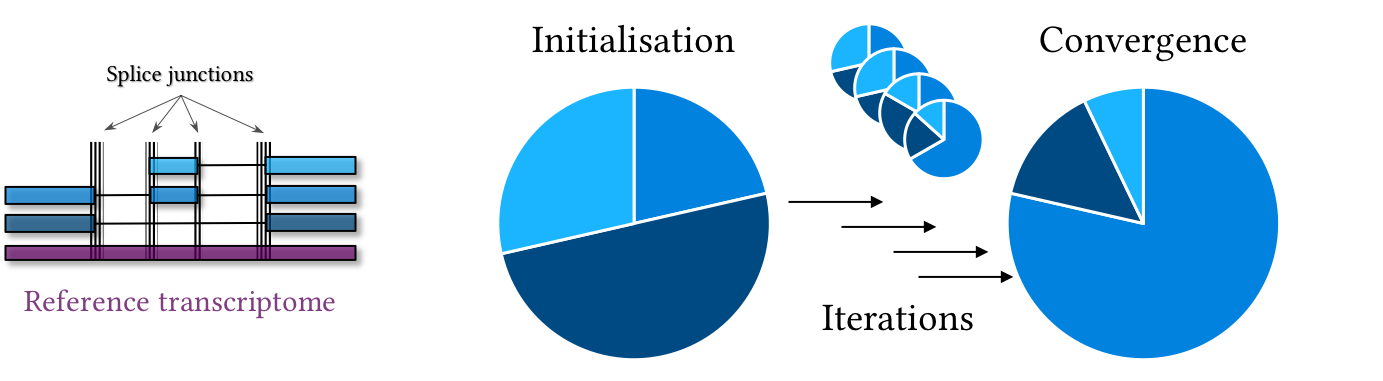
\includegraphics[scale=0.60]{introduction/CufflEstimation.png}\centering
    \caption[Abundance estimation of isoforms by
    Cufflinks]{\label{fig:cuffEstimation}\textbf{Abundance estimation of isoforms
    by \cuffl} following an \gls{EM} algorithmic approach. [Adapted
    from~\cite{Turner2015}]}
\end{figure}

Finally, to compute the gene expression levels, \cuffl\ aggregates \latin{per}
gene all the isoforms expression abundances together.

\NB\ \cuffl\ provides by default \FPKM\ \emph{normalised} data (see
\cref{subsub:norm}).
\minisec{HTSeq-count}
The \gls{Python} library \soft{HTSeq} provides a stand-alone script
(\htseq) performing the feature quantification with a more conservative strategy.
It discards all ambiguous reads from a \gls{SAM}/\gls{BAM} file and then
only counts the \emph{un}ambiguous reads that overlap with the features of
interest for a given gene model\footnote{Gene models are distributed as
annotation file (usually either as \gls{GTF} or \gls{GFF} format) and refer
to a specific reference (genome or transcriptome).}.

\begin{figure}
    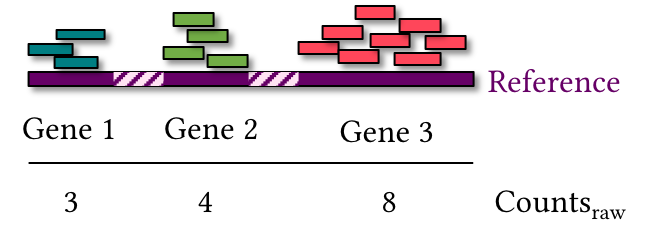
\includegraphics[scale=0.60]{introduction/htseqQuant.png}\centering
    \caption[Abundance estimation of genes by
    HTSeq-count]{\label{fig:htseqEstimation}\textbf{Abundance estimation of genes
    by \htseq}. The unambiguous reads (or fragments if case of paired-end data)
    overlapping locus annotated as gene are directly counted. [Adapted
    from~\cite{MarPhD}]}
  \end{figure}

\htseq\ deems as ambiguous any multiread or read that overlaps more than
one annotation for the considered feature.\footnote{In fact, reads might be
discarded for one feature but kept for another one. For example, to quantify the
expression of a given gene, \htseq\ considers every read that unambiguously
overlaps with any of its annotated exons --- indeed, \htseq\ defines a gene
as the union of all its exons. However, while quantifying exon expression, many
of these same reads may be discarded as they overlap several exon annotations
with overlaying definitions.}
\htseq\ provides
three modes to fine-tune the overlap definition.
For this thesis, I used the \enquote{\texttt{intersection non-empty}} mode
(see \Cref{fig:htseqMode}).
This mode avoids discarding too many reads due to a too tolerant annotation
(\ie\ the annotation itself presents many overlapping definitions for a given
pair of feature and chromosome region).

Initially, \htseq\ was designed for \emph{differential gene
expression analysis} \mycite{htseq}. As multireads are irrelevant for
those studies, including or excluding them from the downstream analysis was
insignificant. Interestingly, many papers
(\eg~\mycite{Fonseca2014,errorsRNAquant,tophatStarwhatever})
have since showed that
the gene expression estimation by \htseq, while underestimated, is overall
well-correlated with other \gls{RNA} quantification methods
(\eg\ microarrays or \gls{RT-qPCR}).

Moreover, quantifications with \htseq\ are highly correlated with \cuffl\
quantifications for most of the genes after proper normalisation
\mycite{tophatStarwhatever} as \htseq\ provides \emph{raw counts} (\ie\
unnormalised counts).


\subsubsection{Normalisation}\label{subsub:norm}
Actually, regardless of the quantification method, a normalisation is usually
necessary to avoid a few statistical biases (mainly due to the sampling). The
normalisation method, though, is generally determined based on the quantification
(method or tool\footnote{Many quantification tools (\eg\ \cuffl) perform
automatically the normalisation step as well. They may also (or not) provide
raw counts.}) and they have to be suitable to the planned downstream analyses.
As unfortunately, \Rnaseq\ lacks (still) to assess the true concentration of each
expressed gene (or transcript) in a sample, each normalisation method is based on
a specific set of assumptions that may be incompatible to the ones required by
a number of investigation approaches.

Many papers review or compare normalisation methods (See~\mycite{Dillies2013,%
normSigCancerHelp,NormImpact,ruvseqComQN}).

\minisec{RPKM and FPKM}
The first evident source of sampling bias is the total number of \emph{mapped}
reads (or fragments) between two \Rnaseq\ libraries (shortened as
\enquote{libraries} from now on). Indeed, there may be huge discrepancies in
their respective amount of starting material loaded on a
\gls{flow}\footnote{In fact, this would involve the monitoring of many parameters
or assessments of the samples before the library preparation. And, while
it \emph{may} be possible to weight each sample before extracting the \gls{RNA},
the many steps (involving the fragmentation of the \glspl{RNA},
\gls{PCR} syntheses or size-selection) and their associated biases
overburden the tracking of the final amounts used for the sequencing.}
and, more importantly, \emph{the amount of mapped reads (or
fragments)} to a reference\footnote{The quantification disregarding the
\emph{unmapped} reads (or fragments) so does the normalisation.}.

The second source of bias arises when two genes have their expression level
compared. Indeed, as a longer gene produces more reads (or fragments), it has
greater stastistical chance to be sampled. \Cref{fig:htseqEstimation} illustrates
this sample bias: \frfig{Gene 3} is twice longer than \frfig{Gene 2} and their
raw counts also present this scaling factor. However, with proper normalisation,
\frfig{Gene 2} and \frfig{Gene 3} are expressed in equal proportions.

To correct for these two biases,~\cite{Mortazavi2008} introduced a new unit
\enquote{RPKM} which they first defined as \emph{\textbf{R}ead} per
\textbf{K}ilobase of \emph{exon model} per \textbf{M}illion mapped \emph{reads}.
From since, this unit is usually redefined as \acrlong{RPKM} and then to
\acrfull{FPKM} to also account for paired-end data\footnote{As mentioned before,
despite the inaccuracy, \emph{read} and \emph{fragment} are often used
interchangeably; this is also the case for \emph{\RPKM} and \emph{\FPKM}.}.

The canonical formula for \FPKM\ (or \RPKM) is:

\begin{equation}
\hat{\mu}_{ij}=\frac{f_i}{F_j\cdot10^{-6} \cdot \ell_i\cdot10^{-3}}
              =\frac{f_i}{F_j\cdot\ell_i}\cdot10^{9} \text{\,}
\end{equation}

where: \\{\small
$\hat{\mu}_{ij}$ is the normalised expression for \emph{feature} (\eg\ gene) $i$
in sample $j$,\\
$f_i$ is the count number of the fragments (or reads) mapped to
\emph{feature} $i$ in sample $j$,\\
$F_j$ is the total count number of all the fragments (or reads) mapped in
sample $j$,\\
$\ell_i$ is the length of \emph{feature} $i$.
}

\NB\ The scaling factor was introduced such as in most cases $1$\ \FPKM\ is
roughly equivalent to $1$\ \gls{RNA} in the cell \mycite{Mortazavi2008}. This
has been observed in other papers (see for example~\cite{Hebenstreit:2011}) and
also explains why $1$\ \FPKM\ is a commonly used threshold.

This normalisation is quite intuitive and still largely used nowadays. In fact,
I use this normalisation through the thesis. However, it is also unsuitable for
a popular type of analysis: \emph{Differential expression analysis}. Indeed,
if a set of genes are expressed in a specific condition and are undetected in
another (either for biological or technical reasons), the \emph{normalised counts}
of every \gls{RNA} in both conditions is then affected (see \Cref{tab:noFPKM4DEA})
and will entangle the interpretation.


\minisec{Other normalisation approaches}
Differential expression analyses (DEA)  have required the development of distinct
models and methods. Indeed, they generally involve a model where for most of the
genes, the expression is stable between conditions\footnote{The comparison is
usually between diseased (or treated) samples to control (healthy).} (\eg\
\soft{edgeR}\footnote{\label{footnote:1}Bioconductor package} \mycite{edgeR}
or \soft{DESeq2}\footref{footnote:1} \mycite{DESeq2}).

Also, a number of normalisation methods applied first to microarrays are used, \eg\
the most common ones include a quantile normalisation method or a simple scaling
normalisation.

Other normalisation methods tries to correct \latin{a priori} or \latin{at
posteriori} biases\footnote{The \gls{BiocR} package \soft{CQN} \mycite{cqn}
for example corrects the expression levels according to their length and
their \emph{GC} content\footnote{\gls{cDNA} enriched in GC bases are stabler and
tend to a more optimal amplification.} before applying a quantile normalisation.}.
A few of them may correct \emph{batch effect} (see \cref{sec:expDesign}) or
other confounding factors. The \gls{BiocR} package \soft{RUVSeq} \mycite{ruvseq}
is one example.

\section{Proteome exploration with Mass spectrometry}

High-throughput protein identification and quantification (\ie\ characterisation)
use \ms\ as the primary method of choice since it allies a good dynamic range
with high sensitivity and specificity \mycite{Aebersold2003,Broshphd,Cox2011}.
Indeed, on the last decade, the field has shifted from technical research on the
instruments and methods to an extensive and routine use of \ms\ as an analytical
tool for life sciences, in particular for proteins \mycite{AebersoldMann2016}.
As \ms\ is very versatile and supports many proteomic investigation
approaches\footnote{E.g.\ Proteome sequences, quantity, modification sites,
structures and context of the protein along with mechanism-oriented
(interaction) studies \mycite{AebersoldMann2016}.},
there are many possible workflows for \ms-based proteomic studies.
As the present thesis focuses only on \gls{DDA} discovery
studies (See \Cref{sec:ProteoData}), I only review the widespread
\emph{bottom-up} approach for identification and quantification
studies\footnote{\emph{Bottom-up approach}: \glsentrydesc{Bottom-up}\\
In fact, \gls{Top-down} approaches while appealing
are still very challenging both as experimental and computational perspectives
\mycite{AebersoldMann2016}.}\sepfootnote\footnote{Bottom-up approaches are
also used for \emph{targeted proteomics} (see \mycite{Shi2016}) and for
\gls{DIA} studies to generate, for instance, comprehensive fragment-ion maps for
specific proteoforms (see \mycite{Chapman2014})}, and more exactly, the
typical \emph{\enquote{shotgun}} proteomics approach that
relies on \gls{LC-MS/MS} \mycite{Cox2011,Zhang2013}. In fact, all
three proteomic datasets used within this thesis are the product of this specific
protocol. The \gls{DDA} approach has many advantages over other approaches
\mycite{AebersoldMann2016}: they are unbiased and free from hypothesis and as
such are great tools for global discovery study. Indeed, \gls{DDA} studies survey
all the proteome at once and prior knowledge is unrequired. The lately increased
popularity of this method%\footnote{First introduced by \cite{Hunt1992}}
~relies on the increased availability of high-quality genome and gene sequence
databases and more recent technical advances in \ms\ (development of new
protein/peptide ionization and fragmentation methods)
\mycite{Aebersold2003,Cox2011,Zhang2014}. In the same manner as for the \Rnaseq,
I will emphasise the techniques used in the aforementioned proteomic datasets.

\subsection{Sample preparation}
Protocols to prepare samples for proteome analyses are quite simpler than the
ones for \Rnaseq. However, as proteins are also more complex and heterogeneous in
nature than \DNA\ and \RNA\ \mycite{Bruce2013}, there is a wider choice of them
in order to adapt to any requirement \mycite{Feist2015}.

\subsubsection{Sample collection and conservation}
\minisec{Collection}
\cite{Feist2015} report that traditional dissection, biopsies, blood draws and
other additional methods can deliver adequate samples for proteome analysis.

\minisec{Conservation}
Recent developments have significantly improved proteome analysis from
\gls{FFPE} samples \mycite{Steiner2014}. Actually, as they are still evolving,
they may compare soon to fresh-frozen (\gls{FF}) samples.
However, for now fresh or \gls{FF} samples are still remaining the best initial
sources.

\subsubsection{Protein extraction and contaminant removal}
\minisec{Protein extraction}
Contrariwise to the collection step,~\cite{Feist2015} explain that the crucial
consideration is the cell lysis and the extraction approaches used on
the protein as they may interact and disrupt the later characterisation step and
thus require appropriate picking. In addition, the physico-chemical properties of
the proteins are far more heterogeneous than for \DNA\ or \RNA\ molecules
\mycite{Bruce2013} and may be incompatible to a number of extraction protocols.

\minisec{Contaminant removal}
\cite{Gutstein2008,Bodzon-Kulakowska2007,Visser2005,Hilbrig2003} review various
examples of mechanical and chemical extraction and contaminant removal methods.
Indeed, contaminants and detergents requires to be eliminated from the samples
before analysis as, in the typical \gls{Bottom-up} approach, they interfere
with the digestion, the separation and fragmentations steps; precipitation and
filtering (based on molecular weight cut-off) strategies are the best in the
context of \gls{Bottom-up} \ms\ analysis \mycite{Feist2015}. Indeed, many
extraction solvents are inappropriate for \ms. Precipitations may denature the
proteins, but this is usually irrelevant in this situation.~\cite{Feist2015}
review different precipitation protocols and emphasises that caution is needed
for the next re-suspension step to avoid missing a consequent part of the
sample proteome. They list several techniques and approaches to this regard.

\subsection{\enquote{Simplification} of the samples}

High-throughput bottom-up workflows (including \gls{LC-MS/MS}) generally
aim to decrease the sample complexity to analyse while increasing the depth
of proteomic coverage \mycite{Zhang2014,Bruce2013,Cox2011}. Indeed,
many aspects may impede the characterisation of the proteins.
For example, the wide physico-chemical property scope of the proteins will
require various protocols to be handle efficiently.
Their concentrations in a sample may saturate the \ms\ characterisation capacity
as the very abundant proteins are easily detected and quantified while rarer
proteins may be missed entirely without specific precautions
\mycite{Liu2009,Cappadona2012} or without unbearably increasing the
analysis time per sample \mycite{Nilsson2010}.

Hence, the usual workflow will usually involve the denaturation, the reducing,
the alkylation and the digestion of the proteins. The peptide mixture products
are then separated in smaller fractions before subjection to \ms\ so to increase
the coverage depth while keeping a reasonable analysis time-frame
\mycite{Aebersold2003,Cox2011,Zhang2013}.

\NB\ The various \emph{simplification} steps may happen in a different order
than I report hereinafter; they may also happen concomitantly. Additionally,
protocols may skip or inversely involve several times the same type of
simplification step. For example, protocols may present a first step of
\emph{proteins} fractioning and then a later step of \emph{peptides} fractioning.

\subsubsection{Denaturation, Reduction and alkylation}

Theses steps may happen simultaneously to other steps. For example, they may
occur while the extraction, the depletion or the digestion. They help to protect
the proteins from endogenous proteases and separate the protein complexes. They
also help to the relative linearisation of the proteins and to some extent to
the homogenisation of the crude mixtures \mycite{Feist2015,Bruce2013}.

\subsubsection{Depletion of highly abundant proteins}

Regrettably, the proteomic field lacks amplification method and
there are very few strategies to remove the highly abundant proteins. Fortunately,
these are very limited in number and may be precisely targeted.
\cite{Zhang2014} reports two useful strategies. The first one aims to remove
them completely from the sample, either by selective
precipitation or by (more expensive) specific antibody-arrays.
The second approach aims to the equalisation of the proteome.
It may be based either on combinatorial ligand libraries involving
bead-supported ligands (on a similar model to \Rnaseq\ protocols)
or on specific protease mixtures\footnote{The former method uses bead-conjugated
hexapeptide ligands to capture (approximatively) equimolar amounts of proteins.
The very abundant proteins will bind till saturation to the beads and their
remaining part in solution are washed off. This cheaper method has drawbacks.
For example, it presupposes that every protein has a corresponding ligand to bind.
\\\cite{MichaelMentenDepletion}, for example, describes the later method. The
key of this protocol is to digest the most abundant proteins into peptides while
keeping the bulk of the other proteins intact. Then, a filtering (based on
molecular size) removes the peptides.}.

In general, the equalisation of the proteome improves the characterisation
of the scarcer proteins \mycite{Zhang2014} while they may introduce skewness
to the analyses (due to the relative protein proportions).

\subsubsection{Proteolytic digestion}
It may seem contradictory to digest the proteins into peptide mixtures as a mean
of \emph{simplification} step. And yet, while the main drawback is the inability
to distinguish between proteoforms \mycite{Bruce2013}, it improves the proteins
characterisation on several points.
\begin{itemize}
    \item It helps to homogenise the sample: peptides present closer
        physico-chemical properties to each other than proteins \mycite{Zhang2014}.
        In addition, peptide separations (by gel or \gls{LC}) are easier than
        for proteins (see \cref{subsub:sepMethods}).
    \item \ms\ is also more sensitive to the peptides than to the proteins as
        \ms\ is more sensitive towards lower molecular-weight molecules
        \mycite{Vitek2009,Cox2011}. Proteins may also be too large to be
        fragmented (\eg\ with \gls{CID}) \mycite{Bruce2013}.
    \item It is also easier to accurately characterise (identification and
        quantification) smaller molecules. In fact, large proteins with alike
        compositions present very similar molecular mass and may be impossible
        to discriminate. On the other hand, a sequence-specific enzymatic
        digestion gives hints on the protein sequence.
    \item Finally, it increases the coverage of the less abundant proteins
        \mycite{Zhang2014}. Indeed, each protein is represented by multiple
        peptides hence increasing the sampling probability. Often, one or a small
        number of \gls{LC-MS/MS}-characterised peptides is enough to identify the
        parent protein \mycite{Bruce2013}.
        Furthermore, as mentioned previously, a well-designed digestion can deplete
        the final mixture of abundant proteins.
\end{itemize}

The digestion may happen in-gel or in-solution. Both are very well-used.
In-gel digestion is very common in bottom-up approaches based on \gls{LC-MS/MS}
as it provides also directly the fractioning and it is better adapted to more
complex samples. Often, the gel will contain, in addition to the protease, a few
chemical reagents that handle other step (\eg\ chaotropic reagents to denature
the proteins at the same time). However, it requires greater time and amount of
starting material than for the in-solution digestion. In-solution digestion
on the other hand is the simplest and the most widespread
digestion approach among all the proteome studies in general. It usually
foreshadows filtering and fractioning steps. More recently, a hybrid method
combining both method has been developed and named \acrfull{FASP}
\mycite{Manza2005,Wisniewski2009}.

Although there are other enzymes for restrictive digestion, trypsin is the gold
standard protease \mycite{Zhang2014}. Its popularity is also explained by
circularity: as more studies are using it, more data are available for comparison,
hence more studies use it.

\subsubsection{Separation methods (fractioning)}\label{subsub:sepMethods}
Fractioning is the principal method to simplify sample complexity. It also allows
to focus selectively on subcellular fractions when needed. Indeed, one may want
to study in particular organelles, cell compartments or other kinds of proteome
(\eg\ phosphorylated or glycosylated proteins) \mycite{Cox2011}.

Several methods may fraction peptide mixture. Protocols may involve many of their
various combinations. However, the sequential use of a gel and a \gls{LC} is
the most common on unknown complex peptides (or proteins) mixtures before
\ms\ analyses.

\minisec{Precipitation}
They are very easy to perform and they usually involve solvent gradients. While
their use is frequent for desalting crude mixtures, it is also quite limited
for protein mixtures as other separation methods (based either on gel or
capillarity such as \gls{LC}), are more performant.

\minisec{Gel electrophoresis based separation}
Many protocols involve a first gel-based separation method prior to the
liquid-based separation and fragmentation of\enspace\gls{LC-MS/MS}
\mycite{Feist2015}.

The gel separation may comprised one step or two, which are respectively referred
as one-dimension (1D) and two-dimensions (2D) gels.

The widespread sample preparation for bottom-up proteomics is a 1D-gel approach.
It comprehends a denaturing alkylating gel (usually \gls{SDS-PAGE} but other are
possible, \eg\ \gls{LDS-PAGE}) \mycite{Shevchenko2006}. Thus, the proteins lose
all their quaternary, tertiary and secondary structures. The separation relies
then on the length of the proteins. Indeed, \gls{SDS} molecules are negatively
charged and they bind to the proteins proportionally to their length and as an
electric field is applied to the gel, the proteins migrate towards the positive
side of the gel at different speeds due to their difference in their mass-charge
ratio. This 1D protocol is more common than the 2D as it is faster. The later is
usually more selective as it relies on very similar principles but in two separate
steps\footnote{Usually, the proteins are first separated based on their
isoelectric point in a \emph{native} gel (as opposed to a denaturing one).
In fact, an \gls{ampholyte} reagent is added to the gel which ensure a stable
gradient of \gls{pH} through the gel. The proteins migrate till they reached a
\gls{pH} region where their overall charge is neutral. In a second time, the
proteins are separated perpendicularly this time on their mass after the addition
of \gls{SDS} or an alike reagent.}.

Note that a protease may be added to the gel and then peptides are separated
instead.

\minisec{Liquid chromatography (LC)}

Chromatography is a technique of choice for the separation of mixtures into their
components or --- at least --- in simpler mixtures. \gls{LC}, as any kind of
chromatography, involves a \emph{mobile} and a \emph{stationary} phase.
The mobile phase comprises an eluent (\ie\ a solvent) and the mixture to be
separated. A column plays the stationary phase part. To fasten the process, high
pressure may be used (\eg\ \glsxtrfull{HPLC} or \glsxtrfull{UPLC}).

The separation relies on the difference of affinity of the mixtures components
towards the mobile and stationary phases. Many combinations may be used. However,
any inadequate choice may precipitate the mixture on the (\emph{extremely})
expensive column which means that both the column and the mixture will be lost.
Hence, in discovery mode and for complex mixtures (as for proteins extracts),
instead of using a \emph{normal phase}, \ie\ crude silica-gel, column (which
interacts tightly with polar molecules such as peptides and may prevent them to
interact with the mobile phase afterwards), a \emph{reversed phase} column
is more common. In these columns, the silica-gel is modified and has been
attached to long hydrocarbon chain. Thus, the column is unable to fix anything
permanently. Along with a \gls{RPLC} column, polar eluants are used. These
interact strongly with charged proteins and peptides. Hence, the separation
occurs on the polarity of the molecules and the most hydrophobic a molecule,
the longest it will remain in the column as it will present fewer interactions
with the eluent.

The ease of coupling this powerful method to the (also powerful) \ms\ explains
why \gls{LC-MS} is so widespread nowadays. Their combined use also allows high
repeatability and optimised running time.

\subsection{Characterisation through Fragmentation profiles}

The first reported use of the principle underlying \ms\ happened in 1913 when
Sir Joseph John Thomson channelled a stream of neon ions trough an electromagnetic
field and captured its deflection on a photographic plate \mycite{Thomson1913}.
Arthur Dempster built a first mass spectrometer in 1918. Francis  William
Aston (Thomson's student) created his own complete one in 1919 \mycite{Aston1919}.
\begin{comment}
\ms\ became rapidly a pillar
of the so-called \emph{modern analytical techniques} in Chemistry as it allows
for a large spectrum of molecules of interest, the detection,
the characterisation and even, for the smaller ones, the resolution of their
structures.
\end{comment}
In this context, the use of \ms\ in proteomics is quite recent as it
is developing from the 1980s onwards \mycite{BiomolBio}.

\subsubsection{General principle}

\ms\ relays on the following principle: molecules of interest are ionised
into charged particles then the mass analyser separates them in the gas phase
based on their total mass $(m)$ to charge $(z)$ ratio, \ie\ $m/z$.
A detector collects all these ions and translates their signal (intensity versus
$m/z$) to an electric one which is the output serving as raw data for the
later analyses. In the simpler case, the molecules are singly charged ($z=1$) and
their molecular mass is only recorded. However, it is quite common for the
molecules to carry more than one electric charge and that if the energy used for
the ionisation is substantial, they may also forego fragmentation and internal
reactions that will result to the production of many spectra. The collection
of spectra obtained from a single peptide ultimately increase the accuracy of
the mass measurement and the identification of the peptide \mycite{BiomolBio}.
Indeed, these peptide-mass profiles are a very effective way to identify
proteins in a very short laps of time as long a reference database is available
for the studied organism \mycite{Pappin1993}. The recent completion of the human
genome sequence and many other organisms has accelerated the general use of this
analytical method \mycite{Luge2016}. In addition, recent developments have
showed that the use of two mass spectrometers in tandem (\gls{MS/MS}) reduces
significantly the number of missed proteins while keeping reasonable running
times and it is more powerful than excessive fractioning as is the improvement
of \gls{HPLC} \mycite{Cox2011}.

\subsubsection{Ionisation}

While there are other methods (more adapted to small organic molecules)
two \emph{soft} ionisation methods are routinely used for proteomic samples:
\acrfull{MALDI} and \acrfull{ESI}.

\gls{MALDI} is very useful for large molecules. It allows to create ions with a
minimum of fragmentation (if none at all). The molecules are fixed on a matrix
(a gel) and then a pulsed \gls{laser} irradiates the sample which provokes the
ablation and then the desorption from the matrix and ionisation of the molecules.
This method had an increased popularity as separation gels (\eg\ \gls{SDS-PAGE})
may be used directly for both steps. \mycite{BiomolBio}. However, many
manufactured mass spectrometers are incompatible with this ionisation technique
\mycite{Zhang2014,Walther2010}.

\gls{ESI} is currently the most popular technique of ionisation, particularly
because it may be used with a large panel of different analysers and that it
interfaces efficiently with \gls{HPLC} or \gls{UPLC}. The ionisation is realised
through an electrostatic method. The application of a high electric potential on
a needle through which a liquid (containing the dissolved analyte peptides)
is passing provokes its dispersion into small and highly charged droplets.
These droplets start to evaporate to the point where the charge on their surface
is so high that a desorption of the analytes occurs.  The analytes are then
in an ionised form (often many charges). They are then released into the mass
spectrometer. \mycite{Walther2010}

\subsubsection{Mass analyser}

Many different mass analyser designs are available. They all share two properties:
they accelerated the ions (in a vacuum) so all the ions share the same kinetic
energy and then they deflect (and thus resolve) the ions based on
their various $m/z$.  A number of them are also
capable of trapping and storing specific range of ions for deeper analyses until
they release them based on their $m/z$.
The most common commercial analysers include quadrupole (Q), \acrfull{LIT},
\acrfull{TOF}, ion traps and most recent \gls{FT} analysers such as \acrfull{ICR}
and \orbi. The choice of one analyser over others or any combination of them
depends on many factors (including the ready availability). \mycite{Haag2016}

Hereinafter, I review the analysers involved in the production of the
proteomic raw data used within this thesis. Indeed, all the datasets have been
produced by a combination of \acrfull{LTQ} and \orbi. I also review very
shortly the quadrupole analyser. (See~\cite{Haag2016} for more details on other
types of analysers.)

\minisec{Quadrupole analyser}

It is one of the most popular analyser. In fact, they are cheap compared to the
others. They are also compact, durable and reliable. The quadrupole analyser is
able to filter the ions based on their difference of $m/z$. The are adequately
named quadrupole as they comprise four cylindrical or hyperbolic rods in
parallel of each other. Opposite rods are connected together electrically and
\gls{RF} potential is applied. A \gls{DC} potential is superimposed on the
\gls{RF} one. These combination of \gls{RF} and \gls{DC} potentials constrain the
ions to oscillate between the rods as they pass through them. Hence, by tuning
the \gls{RF} and \gls{DC}, it is easy to select for which range of $m/z$ ions
will have a stable trajectory and thus the only one detected. Indeed, the
ions with unstable trajectory will collide with the rods and be \enquote{filtered}
out. If used in \enquote{\gls{RF}-only} mode (\gls{DC} reduced in a minimum),
the quadripole may have other applications. For example, it can guide specific
$m/z$ ions to other area (while the bulk of ions will remain trapped).
It may also be used as collision cells for \gls{CID}: by introducing an inert
gas and tuning with the \gls{RF}-energy, the amount of fragmentation undergone
by the targeted ions can be precisely controlled. \mycite{Haag2016}
The quadrupole analyser is also qualified as mass filter.

\minisec{\Acrfull{LTQ}}
\gls{LTQ} also called \acrfull{LIT} are in principle a kind of a quadripole
mass analyser. A \gls{LTQ} uses a set of
quadrupole rods and a two-dimensional \gls{RF} field confines the ions radially.
In addition, a static electrical potential is applied to end electrodes which
forbid the ions to escape axially. However, the quadripole is commonly segmented
in three parts which ensures a perfect homogeneity of the electric field of the
trap area and thus avoiding ion loss when the trapping is done.
While they may be used as an ion trap, they
may be also used as a simple mass filter. \gls{RF} voltage is tuned to produce
multi-frequency resonance ejection waveforms are applied as to
eliminate all the undesirable ions in the trap before the fragmentation and mass
analysis of the remaining ones. Frequently, these \glspl{LTQ} are used as a
front-end to other mass analysers as they have high injection efficiencies and
high ion storage capacities. They may be equipped then of two biased radial
ejection slits and then be used with two detectors hence the signal-to-noise
ratio may be doubled.

Compared with other traps, linear ion traps provide an enhanced dynamic range
with a reduced low mass cut-off as the ion cloud is
spatially distributed on a linear axis and not a 3D centre which improves the
sensitivity. And then, for example, the ions may then be accumulated before
being released into another mass analyser \mycite{Madalinski2008}.

\minisec{\orbi}
It is a very recent analyser and it relies on \gls{FT}. Recently,
there is an increasing use of \glspl{FTMS} for proteomic studies. Indeed, these
\glspl{FTMS} are more precise than previous analysers and allow the detection of
a greater range of ions in very short lapses of time \mycite{Scigelova2011}.
In this kind of analyser, ions are trapped and both orbit around and oscillate
in an electrostatic field between an inner and outer part of a central electrode
shaped as a spindle. The ions can only move following the spindle long axis
\mycite{Makarov2000}. While moving around the spindle the ions create a current.
Images of this current are recorded by the outer part of the spindle and after
Fourier transformation of these images allow to obtain very high mass accurate
and high sensitive mass spectra for a greater dynamic range than most of the
other analysers. \mycite{Hu2005}

\minisec{\gls{LTQ}-\orbi}
It is an hybrid (tandem) mass spectrometer that has a \gls{LTQ} as a first MS$^1$
and an \orbi\ as MS$^2$. This \gls{MS/MS} enables multiple levels of
fragmentation for the elucidation of a wide range of peptides and can be coupled
with an \gls{ESI} which is a continuous source of ionisation. This instrument
allows to analyse proteomic samples optimally both in terms of starting material,
time \mycite{Scigelova2011} and provides \enquote{ultrahigh} mass resolution,
high mass accuracy and enhanced dynamic range with respect to mass accuracy
\mycite{Madalinski2008}.

\subsubsection{Fragmentation techniques \mycite{Zhang2014}}

The overall quality and success of peptide (and then proteins)
identification depends largely on the quality of ion fragmentation. To improve
the identification of the peptides, the number of fragmentations are increased,
but in a rather clever way thanks to \gls{MS/MS} use. Indeed, the first \ms\ is
used to select specific ions (hence known $m/z$) to pass to a second \ms.
Thus for each \emph{precursor} ion, a collection of fragmentation mass spectra
can be gathered. The peptide sequences are then more likely to be accurate and
the risk of false positive is significantly decreased.

While in many cases, the experimenter may want to limit fragmentation, they may
also use devoted techniques to increase it. There are schematically different
classes of fragmentation techniques: a collisional, an
electron-based a photon-based. In the collisional category, \gls{CID},
mentioned previously, is a very common one. The chosen ion is introduced in the
collision cell and when it collides with a particle of the inert gas, its kinetic
energy is transformed into internal energy. The fragmentation happens when this
internal energy is enough to activate the dissociation of the ion. Another
related and slightly more effective method for higher charge state ions is the
\acrfull{HCD}. This latest method has gained popularity with the development of
quantitative proteomics (\eg\ \gls{iTRAQ}) has it provides in parallel peptide
identification and quantitation. In the electron-based category, there is the
\acrfull{ETD} technique. In \gls{ETD}, an anion donates an electron to a cationic
peptide. The backbone of this peptide will then fragment \mycite{Syka2004}.
For the other categories, see the review from \mycite{Zhang2014} and the included
literature.

\subsection{Bioinformatic strategies for proteomics studies}

\ms-based proteomics is quite challenging and the major bottleneck of
proteomics pipelines remains the data analysis \mycite{Chen2016}. There are
various tools for proteomics analysis (as there was for \Rnaseq) and they may
be combine in many different pipelines.

\subsubsection{From peptide identifications to proteins}


\minisec{Detecting peptide peaks}

\minisec{Database of candidate peptides}

\minisec{Scoring function}

\minisec{Search Algorithm}

\minisec{False Discovery Rate (FDR) of spectral identification}

\minisec{Protein inference}

\subsubsection{Quantification}

\minisec{Signal Processing}

\minisec{Transformation, normalisation and summarisation}

\minisec{Learning}





\section{Reproducibility and Experimental design}\label{sec:expDesign}
    \subsection{Batch effect}\label{sub:BatchEffect}
    Batch effect: \mycite{batchEffect}
    \subsection{Technical replicates}
    \TK{definition: technical replicate}
    \subsection{Biological replicates}
    \TK{definition: biological replicate}
    \subsection{Bioinformatic pipeline}

\begin{comment}
\begin{itemize}
            \item{Different samples}
            \item{Technology: wet lab but also software: Rupgrade, \ldots}
            \item{missing meta-data}
        \end{itemize}
    \subsection{Main concerns}
        \subsubsection{Detection}
        \subsubsection{Quantification}
    \subsection{Consistency through biological layers}
\end{comment}


\mycite{reviewRNAseqBestpractice}



\section{`Conclusion'}

\begin{comment}
\Rnaseq\ as \Dnaseq\ needs many corrections as to prevent biases in the downstream
analysis. However, due to the dynamic component of the transcriptome
contrarily to the genome, while it is possible to apply the corrections in
\Dnaseq\ and then analyse the data \mycite{dnaseqCorr},
in \Rnaseq, corrections are already part of
the analysis and requires often as much skills than flair. It is possible that
future protocols will overcome this issue.
\end{comment}

\section{Aims of the thesis}

One main focus of my work for this thesis was to appraise the
consistency of findings that have been enlightened in normal Human tissues by
individual large scale transcriptomics and, more recently, large-scale
proteomics studies.

While the amount of data to process and integrate can be challenging,
paradoxically the data available to draw statistically significant conclusions
is often still too sparse. However, we do have enough to provide at least a
qualitative assessment of the consistency and evaluate the feasibility of a
quantitative assessment in general, if not, realise a quantitative integration
for a few key tissues.

\subsection{Achievements}
\begin{itemize}
    \item First time so many datasets have been reprocessed together with the
        same annotation and hence comparison are better (y'a le truc de chez Burges,
        mais ils se sont concentré sur une petite partie des genes)
    \item surtout comparison of Gtex and Uhlen (aussi approfondi)
    \item reprocessing of all the proteome untargeted in human
    \item comparison entre protein expression and 2 datasets (meilleur que le
        science report dans le sens où il y a pas de polémique)
    \item siteweb//application de visualisaiton de la comparison
    \item liste croisé de tissues specifique et house keeping à travers datasets
        transcriptomic et protoemic
    \item attempt de normalisation basée sur les housekeepings
\end{itemize}
